%%%%%%%%%%%%%%%%%%%%%%%%%%%%%%%%%%%%%%%%%%%%%%%%%%%%%%%%%%%%%%%%%%%%%%%%%%%%%%%%%%%%%%%%%%%%%%%%%%%%%%%%%%%%%%%%%%%%%%%%%%%%%%%%%%%%%%%%%%%%%%%%%%%%%%%%%%%
% This is just an example/guide for you to refer to when submitting manuscripts to Frontiers, it is not mandatory to use Frontiers .cls files nor frontiers.tex  %
% This will only generate the Manuscript, the final article will be typeset by Frontiers after acceptance.   
%                                              %
%                                                                                                                                                         %
% When submitting your files, remember to upload this *tex file, the pdf generated with it, the *bib file (if bibliography is not within the *tex) and all the figures.
%%%%%%%%%%%%%%%%%%%%%%%%%%%%%%%%%%%%%%%%%%%%%%%%%%%%%%%%%%%%%%%%%%%%%%%%%%%%%%%%%%%%%%%%%%%%%%%%%%%%%%%%%%%%%%%%%%%%%%%%%%%%%%%%%%%%%%%%%%%%%%%%%%%%%%%%%%%

%%% Version 3.4 Generated 2018/06/15 %%%
%%% You will need to have the following packages installed: datetime, fmtcount, etoolbox, fcprefix, which are normally inlcuded in WinEdt. %%%
%%% In http://www.ctan.org/ you can find the packages and how to install them, if necessary. %%%
%%%  NB logo1.jpg is required in the path in order to correctly compile front page header %%%

\documentclass[utf8]{frontiersSCNS} % for Science, Engineering and Humanities and Social Sciences articles

\usepackage{amsmath,amssymb,booktabs,url,hyperref,lineno,listings,microtype,subcaption}

% Automatic formatting of SI units
\usepackage[binary-units]{siunitx}

\usepackage[onehalfspacing]{setspace}

% Required for 'straight' quotes in code listings
\usepackage[T1]{fontenc}

% Visible TODO notes
\newcommand{\todo}[1]{\textbf{\textsc{\textcolor{red}{(TODO: #1)}}}}

\lstset{language=C++,showstringspaces=false,basicstyle=\tiny,upquote=true}

\linenumbers


% Leave a blank line between paragraphs instead of using \\


\def\keyFont{\fontsize{8}{11}\helveticabold }
\def\firstAuthorLast{Knight and Nowotny} %use et al only if is more than 1 author
\def\Authors{James C Knight\,$^{1,*}$, Thomas Nowotny\,$^{1}$}
% Affiliations should be keyed to the author's name with superscript numbers and be listed as follows: Laboratory, Institute, Department, Organization, City, State abbreviation (USA, Canada, Australia), and Country (without detailed address information such as city zip codes or street names).
% If one of the authors has a change of address, list the new address below the correspondence details using a superscript symbol and use the same symbol to indicate the author in the author list.
\def\Address{$^{1}$Centre for Computational Neuroscience and Robotics, School of Engineering and Informatics, University of Sussex, Brighton, United Kingdom }
% The Corresponding Author should be marked with an asterisk
% Provide the exact contact address (this time including street name and city zip code) and email of the corresponding author
\def\corrAuthor{James C Knight}

\def\corrEmail{J.C.Knight@sussex.ac.uk}


\begin{document}
\onecolumn
\firstpage{1}

\title[Running Title]{Article Title} 

\author[\firstAuthorLast ]{\Authors} %This field will be automatically populated
\address{} %This field will be automatically populated
\correspondance{} %This field will be automatically populated

\extraAuth{}% If there are more than 1 corresponding author, comment this line and uncomment the next one.
%\extraAuth{corresponding Author2 \\ Laboratory X2, Institute X2, Department X2, Organization X2, Street X2, City X2 , State XX2 (only USA, Canada and Australia), Zip Code2, X2 Country X2, email2@uni2.edu}


\maketitle


\begin{abstract}

%%% Leave the Abstract empty if your article does not require one, please see the Summary Table for full details.
\section{}
Inspired by the distributed nature of memory and computation in the brain, neuromorphic systems are designed to provide a more energy-efficient substrate for emulating spiking neural networks when compared to simulations running on Von Neumann architectures.

While neuromorphic systems may be the ultimate platform for \textit{deploying} spiking neural networks, their very distributed nature makes them unwieldy tools for \textit{developing} SNN models.
Instead development and simulation of SNN models tends to be performed on computers with standard Von Neumann CPU architectures and, once models scale above a certain size, clusters of these machines.
However over the last decade, as well as becoming a common fixture in many workstations, NVIDIA GPU accelerators are now used in \SI{50}{\percent} of the Top 10 super computing sites to increase peak performance while lowering power requirements.
In many ways, the large amount of available parallelism and the Single Instruction Multiple Thread (SIMT) architecture of GPUs is well suited to simulating large numbers of homogeneous neurons and synapses, however 
\todo{argument for using GPUs for SNN}

In this paper we re-implement two large-scale point neuron network models with levels of connectivity and sparseness matching those in the neocortex using our GeNN code generator, discussing how they are mapped to GPU hardware.
We then verify the correctness of our GPU simulations before comparing the performance and energy usage against published data for traditional CPU-based HPC as well as neuromorphic hardware where it is available.
We show that a full-scale model of a cortical column can be simulated at speeds approaching $0.5\times$ real-time using a single NVIDIA Tesla V100 accelerator -- faster than is possible using a CPU based cluster or the SpiNNaker neuromorphic system.
Additionally we show that, across a range of GPU systems, the energy per synaptic event is less than half that of a CPU-based simulation and, on a Jetson TX2 embedded system, 

\tiny
 \keyFont{\section{Keywords:} GPU, high-performance computing, parallel computing, accuracy of simulation, energy to solution, benchmarking, computational neuroscience} %All article types: you may provide up to 8 keywords; at least 5 are mandatory.
\end{abstract}

\section{Introduction}

\begin{itemize}
    \item Neuromorphic hardware families - limitations, scales etc
    \item HPC - Neuron, NEST etc, recent benchmarks
    \item GPU hardware introduction - blocks, global memory, L2 cache, shared memory etc
    \item Other GPU simulators - CARLsim, NEURON/Arbor via 3rd party library, NeMo
\end{itemize}

Since the end of ``the free lunch'' -- the point at which it became impractical to continue building ever faster and more complex single-core CPUs -- the only way processor designers have been able to extract more performance from the increasing number of transistors offered by newer fabrication technologies was by build multi-core CPUs. \todo{citations}
However parallel CPU programming paradigms such as multithreading are not well-suited to the type of \textit{fine-grained} parallelism required to harness hundreds of cores.\todo{citations}

The SIMT programming model architecture used by NVIDIA GPUs is designed explicitly for fine-grained parallelism and high throughput.
However spiking neural networks are not especially well-suited


\section{Material and Methods}
\label{sec:method}
\subsection{GeNN}
\begin{itemize}
    \item GeNN code generator - while CUDA is relatively simple, efficiently parallelising SNN code is non-trivial    
\end{itemize}

GeNN neuron models are defined by writing a class defining the model parameters and snippets of C-like code that describe how it should be simulated.
For example the following \lstinline{LIF} class describes a very simple leaky integrate-and-fire neuron with normalised units, solved algebraically:

\lstinputlisting[firstline=2,lastline=15]{code_snippets.cc}

The \lstinline{DECLARE_MODEL} and \lstinline{IMPLEMENT_MODEL} macros insert boilerplate code used subsequently for defining parameters and initial model states in a type-safe manner.
The \lstinline{SET_SIM_CODE}, \lstinline{SET_THRESHOLD_CONDITION_CODE} and \lstinline{SET_RESET_CODE} macros specify the snippets of code used, respectively, to update the simulation state, check whether a spike should be emitted and to reset the neuron after a spike.
The names of model parameters (constant across the entire population) are specified using the \lstinline{SET_PARAM_NAMES} macro and any `pre-processing' logic to be applied to these is specified with \lstinline{SET_DERIVED_PARAMS} -- in this case converting an exponential decay time constant to a multiplier to be applied every simulation timestep.
Finally, the \lstinline{SET_VARS} macro specifies the names and types of the per-neuron state variables.
These macros provide some `syntactic sugar' but are entirely optional -- users can instead override the underlying virtual functions themselves.
In GeNN synapse models are defined using very similar classes with the option to define code snippets for time-driven and event-driven updates.
Event-driven updates can be triggered by pre or postsynaptic spikes as well as by custom events for example the pre or postsynaptic neuron's membrane voltages crossing a threshold.
Once the required models have been defined, the parameters and initial state variables values can be set and \textit{populations} of neurons can be added to a network:
%
\lstinputlisting[firstline=17,lastline=20]{code_snippets.cc}

This listing also illustrate how the approach used for defining models can also be used to define how variables are initialised.
The membrane voltage \lstinline{V} of our \num{1000} LIF neurons is sampled from the uniform distribution using one of GeNN's built in \textit{variable initialisation snippets}.
These are definied in a similar manner to the neuron and synapse models previously described allowing network initialisation to be parallelised uisng the same strategies used for simulating models on the GPU to be applied to initialising their parameters.
This approach is advantageous as it both removes the need to transfer model state from the CPU to the GPU and allows the GPU to be used to accelerate potentially costly initialisation such as sampling random numbers.
%While the PCI express bus typically used to connect the GPU to the host system is relatively fast (up to \SI{16}{\giga\byte\per\second}), initialising millions of synaptic weights on the CPU and then uploading them at the start of the simulation can still considerably slow down the time it takes to iterate the model.
\todo{Benchmark demonstrating speedup from presentation?}

Once network models have been defined using the C++ interface described in the preceding section, GeNN will generate the CUDA code to simulate the network and this can be linked against a simple simulation loop provided by the user:

\lstinputlisting[firstline=22,lastline=32]{code_snippets.cc}

While this approach allows a lot of flexibility and means that visualisation tools and closed-loop robotics can be tightly coupled to GeNN simulations, when combined with the use of C++ for model definition, this does make using GeNN a somewhat daunting prospect to users more used to Python-based simulations such as Brian~\citep{Stimberg2014} or PyNN~\citep{Davison2008a}.
Therefore GeNN offers
\todo{Brian2GeNN, SpineML, PyNN}

\subsection{The cell-type specific cortical microcircuit}
\label{sec:method/microcircuit}
This model of \SI{1}{\milli\metre\cubed} of early-sensory cortex was first developed by \citet{Potjans2012}.
The model consists of around \num{80000} leaky integrate-and-fire~(LIF) neurons, divided into layers 2/3, 4, 5 and 6; where each layer is modelled as an excitatory and an inhibitory population.
Neurons in each population are connected with population-specific densities derived from an extensive review of the anatomical literature resulting in a total of approximately \num{0.3E9} synapses.
In addition to this synaptic input, each neuron in the network also receives independent Poisson inputs with population-specific rates representing input from adjacent cortical regions.
Beside this basic structure, the connectivity is random with both synaptic strengths and transmission delays being normally distributed.
\todo{Thomas: is it necessary to go into further details of network structure or just refer reader to Potjans2012?}
%
\begin{align}
    \tau_{m} \frac{dV_{j}}{dt} = & (V_{j} - V_{rest}) + R_{m}(I_{bias} + I_{s_{j}}) \label{eq:lif_neuron}\\
    \tau_{syn} \frac{dI_{s_{j}}}{dt} = & -I_{s_{j}} + \sum_{i=0}^{n} w_{ij} \sum_{t_{i}^{f}}  \delta(t - t_{i}^{f})\label{eq:exp_neuron_input_current}
\end{align}
%
Although these two state variables are coupled, in our GeNN model, the continuous terms of the two equations are solved separately so the synaptic input current $I_{s_{j}}$ going into equation~\ref{eq:lif_neuron} is effectively treated as a constant during each simulation timestep.
As \citet{Rotter1999} describes, this approach leads to a delay of one simulation timestep compared to the exact solution, but this separation is not only attractive from an engineering point-of-view by better encapsulating the neurons and synapses, but it also provides a generic way of describing neurons with heterogeneous synaptic input dynamics.

Simulating a homogeneous \textit{population} of neurons is an ideal task for a SIMD or SIMT device such as a GPU: the neurons do not communicate with each other and, aside from the relatively rare times that they spike, each neuron will be running exactly the same code.
This means that they can be trivially parallelised by simulating each neuron on a single thread which fetches the neuron's state variables from global memory into registers at the start of each timestep, then advances the simulation state and writes back the state variables.
As long as the state variables are laid out correctly in memory, the required memory operations can be \textit{coalesced} so that a \SI{4}{\byte} state variable can be read for \num{32} neurons in a single \SI{128}{\byte} transaction -- the most efficient way to access the global memory.
%This same parallelism strategy is equally valid for neuron models whose dynamics can only be solved numerically -- the advancing of simulation state simply has to be implemented as for example a Runge-Kutta

\begin{figure}
    \begin{center}
        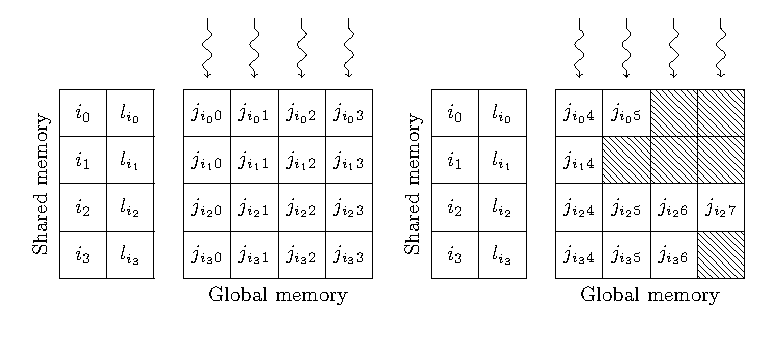
\includegraphics[width=118mm]{figures/ragged_matrix}
    \end{center}
    \caption{GPU parallelism of sparse synaptic matrix processing across two thread blocks each with \num{4} threads.
    Snaking lines indicate CUDA threads.
    Hatching indicates padding entries.}
    \label{fig:ragged_matrix}
\end{figure}

Simulating the sparsely connected synapses between two such populations of neurons is, at first glance, less suitable for GPU parallelism.
However, on modern GPU hardware, this can also be implemented in an efficient manner using the data structures shown in figure~\ref{fig:ragged_matrix}.
This structure consits of multiple 2D arrays where each row represents the synapses coming from a single presynaptic neuron and has enough columns to contain the largest number of postsynaptic targets any presynaptic neuron connects to.
One of these 2D arrays is used to contain the indices of the postsynaptic neurons ($i$) and additional arrays are allocated for any individual synaptic state variables such as the synaptic weight~($w_{ij}$) or dendritic delay~($d_{ij}$).
Each block of $N_{block}$ CUDA threads (in figure~\ref{fig:ragged_matrix} $N_{block}=4$) is responsible for processing $N_{block}$ columns of the matrix.
Processing begins by using the $N_{block}$ thread to fetch the indices of $N_{block}$ presynaptic spikes ($i_{0},\ldots,i_{N_{block} - 1}$) and the lengths of the corresponding rows of the matrix ($l_{0},\ldots,l_{N_{block} - 1}$) into shared memory (as these will be accessed by all threads in the block during the next phase).
Threads are then synchronised and loop through the $N_{block}$ rows with each thread processing the synapse in their column.
In the case of the simple static synapses described by equation~\ref{eq:exp_neuron_input_current} this processing consists simply of reading the index of the postsynaptic target neuron along with the weight $w_{ij}$ and delay $d_{ij}$ associated with the connection and using an atomic add operation to apply the weight to the correct address in the dendritic delay ring-buffer.\todo{say more}
This process is then repeated until all incoming spikes are processed.
While this parallelism strategy may seem counter-intuitive, it typically performs much better than the naïve approach of using one thread per incoming spike as it exposes much more parallelism as well as resulting in perfectly coalesced memory read operations.
For example, if we consider a population of \num{10000} neurons firing at an average rate of \SI{10}{\hertz}, in a \SI{0.1}{\milli\second} timestep it will only, on average, emit \num{10} spikes in a single timestep.
However, if this population is connected to another population with the same size with a \SI{10}{\percent} connection probability, the connection matrix will have over \num{1000} columns resulting in 2 orders of magnitude more parallelism being exposed.

\subsection{Balanced random network with spike-timing dependant plasticity}
\label{sec:method/balanced_random}
The type of one-shot, online learning observed in nature is one of the features of biological neural networks that neuromorphic engineers aspire to emulate.
Synaptic plasticity -- the family of mechanisms responsible for changing the strength of synaptic connections in response to neural activity -- has been shown to be fundamental to learning~\citep{Nabavi2014} and is therefore a key area of computational neuroscience research.
Spike Timing Dependant Plasticity~(STDP)~\citep{Bi1998} is a popular theory which postulates that these changes are driven by the difference in timing between presynaptic spikes arriving at a synapse and the times at which the postsynaptic neuron itself spikes.
In excitatory cortical neurons~\citep{Markram1997} as well as in the hippocampus~\citep{Bi1998}, synapses at which a presynaptic spike is closely followed by a postsynaptic spike are strengthened whereas those at which a postsynaptic spike precedes a presynaptic spike are weakened.
The intuition behind this relationship is that synapses that are implicated in the firing of the postsynaptic neuron are strengthened and those that are irrelevant are weakened.

However, adding STDP to spiking neural network simulations typically increases the computational cost of simulating them significantly. 
\citet{Morrison2007} reported that adding plasticity to their simulations slowed them down by ``a factor of less than 10'' and \citet{Knight2016b} found that, in the \textbf{best} case, simple STDP plasticity reduced the performance of the SpiNNaker neuromorphic system by approximately $6\times$.
Furthermore, the dynamics of neural systems with plasticity operating on biologically-plausible time scales also take several orders of magnitude more time to stabilise.
%Perhaps because of these issues, there are relatively few large-scale network models with synaptic plasticity.
However, \citeauthor{Morrison2007} argue that it is vital to perform experiments on STDP in models with full-scale connectivity, as simplifying connectivity typically results in fewer, stronger incoming synapses per neuron.
These stronger synaptic inputs are then likely to increase the correlation between neurons and, because STDP is inherently sensitive to correlated neural activity, this is likely to cause artefacts in the learned synaptic weights.
Therefore \citeauthor{Morrison2007} developed a large balanced random network model~\citep{Brunel2000} with \num{90000} excitatory and \num{22500} inhibitory neurons -- the scale necessary to achieve realistic connection probabilities of $\approx0.1$ and \num{10000} incoming connections per neuron~\citep{braitenberg2013cortex}.
Balanced random networks have been shown to reproduce some of the dynamics seen in the neocortex~\citep{Brunel1999,Brunel2000} and, by adding STDP, \citeauthor{Morrison2007} showed that STDP does not disrupt these dynamics.

Similarly to the microcircuit model described in the previous section this model uses LIF neurons.
However, rather than exponentially filtering the incoming synaptic input, this model uses a slightly more complex \textit{alpha} synapses \todo{cite} which provide a closer match to the dynamics of biological ion channels:
%
\begin{align}
    \tau_{syn} \frac{dI_{s_{j}}}{dt} = & x_{s_{j}} - I_{s_{j}} \label{eq:alpha_neuron_input_current_1}\\ 
    \tau_{syn} \frac{dx_{s_{j}}}{dt} = & -x_{s_{j}} + \sum_{i=0}^{n} w_{ij} \sum_{t_{i}^{f}}  \delta(t - t_{i}^{f}) \label{eq:alpha_neuron_input_current_2}
\end{align}
%
Aside from requiring an additional state variable to hold $x_{s_{j}}$, equations~\ref{eq:alpha_neuron_input_current_1}~and~\ref{eq:alpha_neuron_input_current_2} are i
As well as alternative synaptic plasticity rules using postsynaptic membrane voltage~\citep{Brader2007,Clopath2010c} rather than postsynaptic spike times and those including `third factors' such as dopamine~\citep{Izhikevich2007}, there are a plethora of different STDP formalisations (see \citet{Morrison2008} for a review).
However, in the model described in this section, \citet{Morrison2007} chose to use a rule with the following relationship between pre~($t_{pre}$) and postsynaptic~($t_{post}$) spike timing ($\Delta t = t_{post} - t_{pre}$):
%
\begin{align}
    \Delta w_{ij} & = \
        \begin{cases}
            \lambda w_{0}^{1-\mu} w_{ij}^{\mu} e^{-\frac{|\Delta t|}{\tau}} & if\, \Delta t>0\\
            -\lambda \alpha w_{ij} e^{-\frac{|\Delta t|}{\tau}}             & if\, \Delta t\leq0
        \end{cases}
\end{align}
%
\section{Results}
\subsection{Correctness}
\citet{VanAlbada2018} performed an in-depth analysis of the correctness of simulations of the microcircuit model described in section~\ref{sec:method/microcircuit} running on both the SpiNNaker neuromorphic system and NEST running in `grid-based' mode.
While the GPU simulations presented in this paper do not face the issues with quantisation which can affect SpiNNaker, unlike NEST, they all use single rather than the double-precision floating point and therefore have the potential for more numerical instability.
Additionally, the non-associative nature of floating point operations mean that, if the results from a large number of parallel threads are summed together in a non-deterministic order, can have large error bounds.
\citet{Villa2009} demonstrated this by calculating Euclidian sums of \num{28000} double-precision floating point numbers across \num{16000} threads of a CRAY XMT system (which, in this context, has similar properties to a GPU) and found that results varied by up to \SI{24.64}{\percent}.
However, in this experiment, more numbers are being summed than any neuron has input and the parallelism schemes described in section~\ref{sec:method} it is unclear what the ranges of the numbers being summed was and
Nonetheless, in this section, we will follow the methodology used by \citet{VanAlbada2018} and compare the results of our microcircuit simulation to those computed using NEST running in `exact integration' mode.
Additionally we will compare the results of simulations of the balanced random network model we describe in section~\ref{sec:method/balanced_random} with those presented by \citet{Morrison2007}.

While the randomisation of the neuron's initial membrane voltages should reduce this, 

\begin{figure}
    \begin{center}
        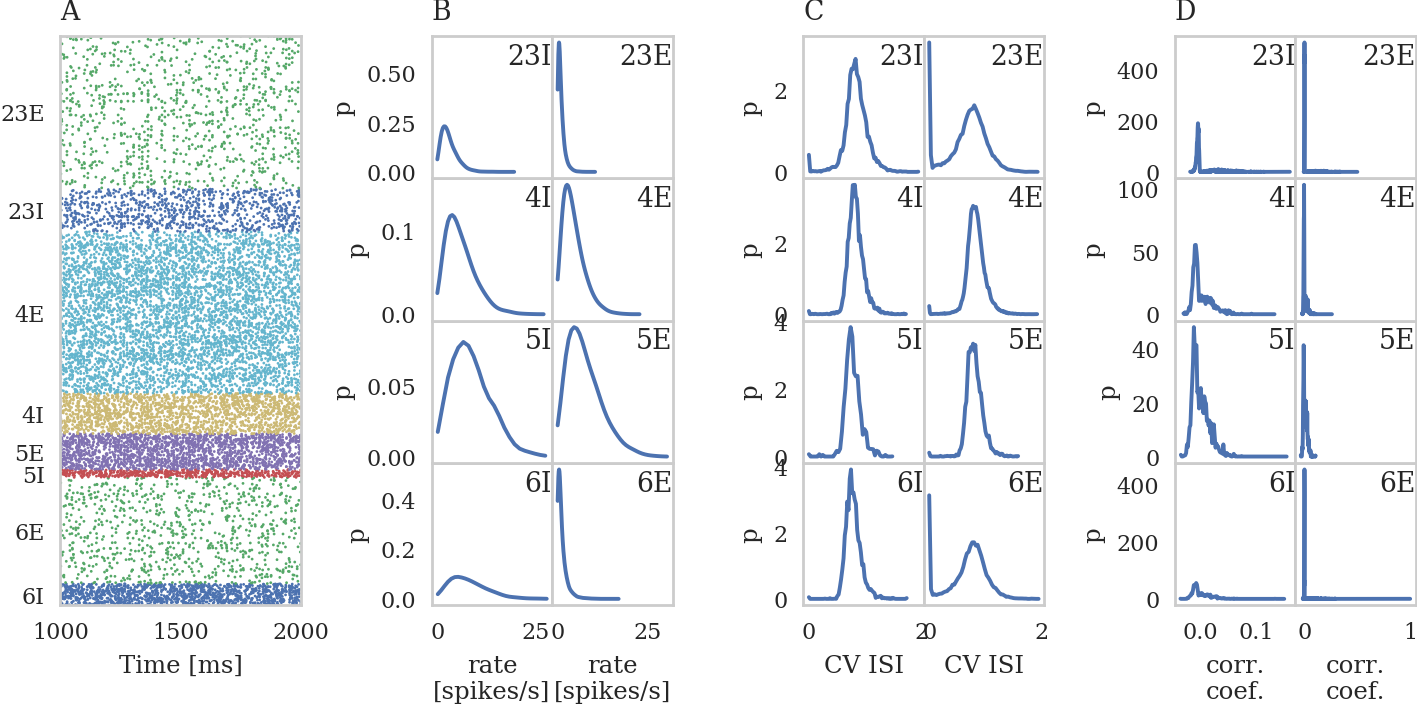
\includegraphics[width=180mm]{figures/microcircuit_accuracy}
    \end{center}
    \caption{Spiking output of cortical microcircuit model with Poisson input.\\
    \textbf{(A)} Raster plot showing spike times (dots) of neurons from each population.
    The spikes of 5\% of neurons (vertical) are shown.\\
    \textbf{(B)} Single-neuron firing rates of all neurons.\\
    \textbf{(C)} CV ISI, a measure of irregularity of all neurons.\\
    \textbf{(D)} Correlation coefficients between binned spike trains for \num{200} neurons in each population.
    All measures are calculated over the last \SI{9}{\second} of the simulation and histogram bin widths are determined using the Freedman-Diaconis rule.}
    \label{fig:microcircuit_accuracy}
\end{figure}

\begin{figure}
    \begin{center}
        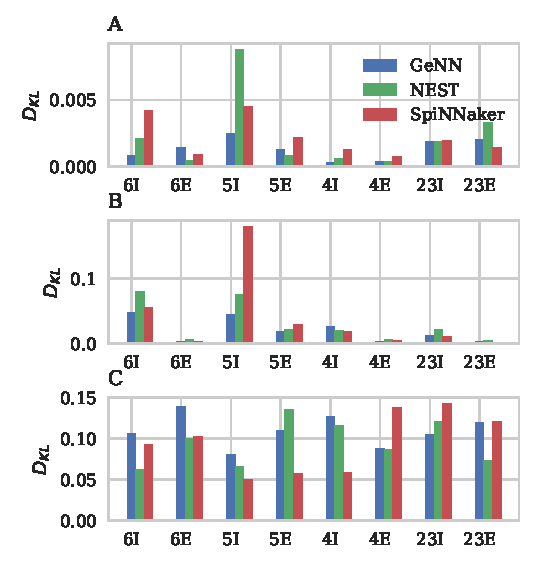
\includegraphics[width=85mm]{figures/microcircuit_accuracy_kl}
    \end{center}
    \caption{Comparison of distributions of microcircuit dynamics including NEST running in `grid-based' mode and SpiNNaker for comparison.\\
    \textbf{(A)} Single-neuron firing rates of all neurons.\\
    \textbf{(B)} CV ISI, a measure of irregularity of all neurons.\\
    \textbf{(C)} Correlation coefficients between binned spike trains for \num{200} neurons in each population.\\
    Comparisons are calculated using the Kullback-Leibler (KL) divergences of the distributions of each dynamics against that calculated from NEST running in `exact integration' mode for each of the 8 populations.
    All measures are calculated over the last \SI{9}{\second} of the simulation and histogram bin widths are determined using the Freedman-Diaconis rule.\todo{what to say about eye-balling from paper}}
    \label{fig:microcircuit_accuracy_kl}
\end{figure}

\subsection{Performance}
\label{sec:results/performance}
To assess the performance of our GPU simulations we chose the selection of GPUs listed in table~\ref{tab:gpu_devices} -- covering a range of financial and power budgets.
CUDA abstracts away the degree of parallelism exposed by the application from the amount of hardware parallelism available so we can run a model that uses \num{80000} threads on a GPU with many fewer CUDA cores.
However memory is a harder constraint and, because of this, while all of the GPUs listed in table~\ref{tab:gpu_devices} can run the microcircuit model described in section~\ref{sec:method/microcircuit}, only the two `Tesla' GPUs have enough memory to run the balanced random network model described in section~\ref{sec:method/balanced_random}.

\begin{table}
  \centering
  \begin{tabular}{r S r S S S S}
    \toprule
        {Model}         & {TDP}             & {Architecture}    & {Num.}    & {Memory}              & {Memory}                      & {Max single-precision}\\
                        & {[\si{\watt}]}    &                   & {CUDA}    & {capacity}            & {bandwidth}                   & {performance}\\
                        &                   &                   & {cores}   & {[\si{\giga\byte}]}   & {[\si{\giga\byte\per\second}]}& {[GFLOPS]}\\
    \midrule
        GeForce 1050 Ti & 75                & Pascal            & 768       & 4                     & 112                           & 2100\\
        Jetson TX2      & 15                & Pascal            & 256       & 4\textsuperscript{1}  & 58.4                          & 600??\\
        Tesla K40m      & 245               & Kepler            & 2880      & 12                    & 288                           & 4290\\
        Tesla V100      & 250               & Volta             & 5120      & 16                    & 900                           & 14000\\
    \bottomrule
  \end{tabular}

  \caption{GPU devices.\\
  \textsuperscript{1}~Memory is shared between CPU and GPU.}
  \label{tab:gpu_devices}
\end{table}

We measured the performance of both models by querying the \lstinline{std::chrono::high_resolution_clock} on the host computer around the simulation loop to get a total simulation time and, in the case of the microcircuit model, around the code used to calculate the connectivity.
Additionally we used CUDA's own event timing system~\citep[Section~8.1.2]{NVIDIACorporation2018} to record the time taken by the neuron and synapse simulation kernels as well as the postsynaptic learning kernel in the balanced random network model.

\begin{figure}
    \begin{center}
        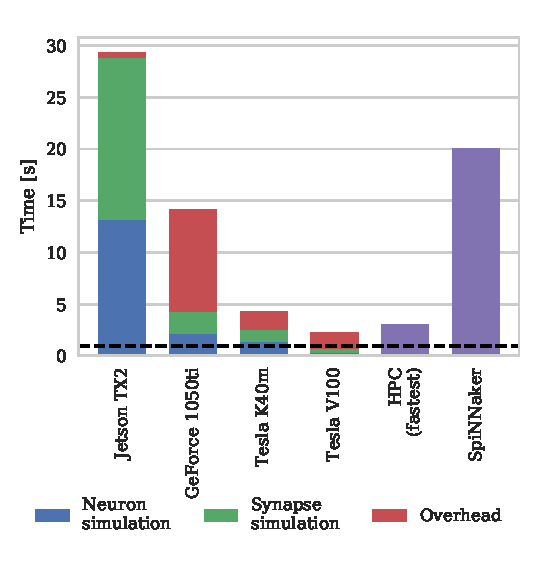
\includegraphics[width=85mm]{figures/microcircuit_performance}
    \end{center}
    \caption{Simulation times of microcircuit model running on various GPU hardware for \SI{10}{\second} of biological time.
    SpiNNaker and fastest HPC simulation times presented by \citet{VanAlbada2018} included for comparison.
    `Overhead' in GPU simulations refers to time spent in simulation loop but not within CUDA kernels.}
    \label{fig:microcircuit_performance}
\end{figure}

Figure~\ref{fig:microcircuit_performance} shows the durations of simulations of the microcircuit model running on each GPU for \SI{10}{\second} of biological time, including the times taken by 

\todo{volta `Independent Thread Scheduling' may be part of the reason why second model works so well}

\begin{figure}
    \begin{center}
        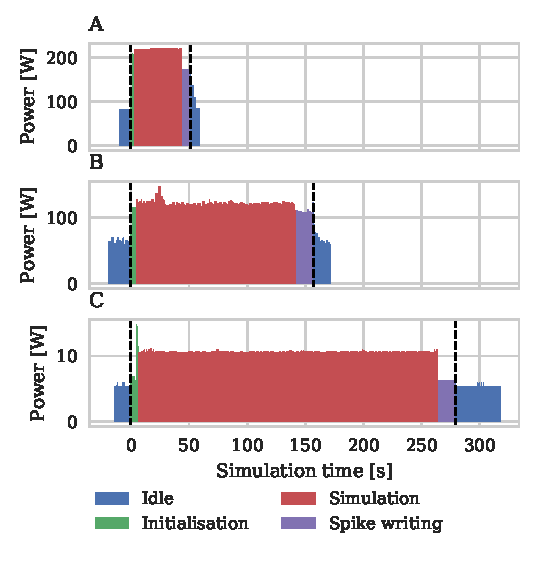
\includegraphics[width=85mm]{figures/microcircuit_power}
    \end{center}
    \caption{Power consumption during \SI{10}{\second} microcircuit simulation.
    Power was measured using consumer power measurement device with minimum resolution of \SI{0.1}{\watt} at mains socket.\\
    \textbf{(A)} GeForce 1050Ti in a desktop PC with an Intel Core i5 750 processor running Windows 7.\\
    \textbf{(B)} NVIDIA Jetson TX2 development kit running Ubuntu 16.04 LTS in maximum performance mode. \todo{figure out JetPack version}}
    \label{fig:microcircuit_power}
\end{figure}

\subsection{Power and energy}
As well as recording the timings of the microcircuit benchmark described in the previous section, we also recorded the power usage of the systems being benchmarked using a consumer power measurement device at the mains socket.
The screen of the power measurement device was recorded using a webcam, optical character recognition was performed using `Seven Segment Optical Character Recognition' developed by \citet{Auerswald2018} and the resultant power measurements were tagged with a time and written to disk.
Figure~\ref{fig:microcircuit_power} shows the power usage over time for simulations of the microcircuit model running for \SI{10}{\second} of biological time on each of the devices listed in table~\ref{tab:gpu_devices} aside from the Tesla V100 which we do not have local access to record the power usage of the entire system.

\begin{table}
  \centering
  \begin{tabular}{r S S S}
    \toprule
        {Model}                 & {Energy to solution}      & {Simulation energy}       & {Energy per synaptic event} \\
                                & {[\si{\kilo\watt\hour}]}  & {[\si{\kilo\watt\hour}]}  & {[\si{\micro\joule}]} \\
    \midrule
        GeForce 1050 Ti         & 0.006                     & 0.0055                    & 2.1 \\
        Jetson TX2              & 0.002                     & 0.00077                   & 0.30  \\
        Tesla K40m              & XXX                       & XXX                       & XXX \\
        SpiNNaker               & {--}                      & 0.017                     & 5.9 \textsuperscript{2}\\
        NEST (lowest energy)    & {--}                      & 0.012                     & 4.4 \\
    \bottomrule
  \end{tabular}

  \caption{Energy cost of simulations.
  Energy to solution and simulation energy of GPU are calculated using the \lstinline{numpy.trapz} and the simulation energy is divided by the total number of synaptic events processed to obtain the energy per synaptic event.
  For comparison, simulation energies for SpiNNaker and NEST are read off the figure presented by \citet{VanAlbada2018}.
  Energies per synaptic event for SpiNNaker and NEST are those reported by \citet{VanAlbada2018}.\\
  \textsuperscript{1}~This energy per synaptic event is calculated after the `idle' power of the SpiNNaker system has been taken into account.}
  \label{tab:energy_measures}
\end{table}

By integrating the power time series using the \lstinline{numpy.trapz} function we we can calculate the energy to solution of each simulation as well as the energy per synaptic event -- a common evaluation measure for the energy efficiency of neuromorphic systems.
\todo{Telsa K40m figures so I can write something meaningful here}
While we were unable to measure the energy of the system containing the Tesla V100 directly, both the Tesla cards have built in power monitoring which showed that the Tesla V100 drew a maximum of \SI{88}{\watt} compared to \SI{107}{\watt} for the Tesla K40m.
Assuming that a Tesla V100 was attached to the same workstation used for the Tesla K40m simulations we can therefore estimate that the total energy to solution would be \todo{XXX} kWh and the energy per synaptic event would be \todo{YYY}.

\section{Discussion}

\subsection{Neurorobotics}
afa

\subsection{Interactive simulation}
asfs

\subsection{Further optimisation and GPU architectures}
The results in section~\ref{sec:results/performance} show that, while the entire initialisation of the balanced random network can be effectively offloaded to the GPU, because the synapses connected using the `FixedNumberTotal' rule have to be initialised on the CPU this adds in the order of \SI{20}{\second} to each microcircuit simulation when run on a workstation or HPC node and almost \SI{10}{\minute} when run on the Jetson TX2.
Initialising this form of probabilistic connector involves a three stage process:
%
\begin{enumerate}
    \item Sampling from a multinomial distribution to obtain the number of connections per row.
    \item For each row, sampling the correct number of indices from a uniform distribution.
    \item Sorting each rows indices into ascending order to improve performance.
\end{enumerate}
%
While the first stage of this process is difficult to parallelise, the second stage is trivially parallelisable and, while sorting is not a particularly GPU-friendly operation, \citet{Awan2016} has shown that simple in-place sorting algorithms such as insertion sort can be used to efficiently sort large numbers of relatively short arrays in parallel on a GPU.
Therefore a hybrid approach where the row lengths are calculated on the CPU and the rows then populated on the GPU is likely to significantly improve performance.

Because the SIMT programming model used by GPUs does not require the complex coherant caches which is making simply adding more CPU cores to symmetric multiprocessing difficult~\todo{citation}, it is expected that GPU hardware will continue to scale~ \todo{citation}.
However, even with new even higher speed memory technologies such as HBM3~\todo{citation}, memory bandwidth has historically always lagged behind processing performance.


\begin{itemize}
    \item Half precision float, ILP - should double performance on TX1
\end{itemize}

\begin{itemize}
    \item HBM3 - further doubling of memory bandwidth
    \item FP16 - half memory bandwidth, double arithmetic throughput
\end{itemize}

\section*{Conflict of Interest Statement}
The authors declare that the research was conducted in the absence of any commercial or financial relationships that could be construed as a potential conflict of interest.

\section*{Author Contributions}
The Author Contributions section is mandatory for all articles, including articles by sole authors. If an appropriate statement is not provided on submission, a standard one will be inserted during the production process. The Author Contributions statement must describe the contributions of individual authors referred to by their initials and, in doing so, all authors agree to be accountable for the content of the work. Please see  \href{http://home.frontiersin.org/about/author-guidelines#AuthorandContributors}{here} for full authorship criteria.

\section*{Funding}
Details of all funding sources should be provided, including grant numbers if applicable. Please ensure to add all necessary funding information, as after publication this is no longer possible.

\section*{Acknowledgments}
This is a short text to acknowledge the contributions of specific colleagues, institutions, or agencies that aided the efforts of the authors.

\section*{Data Availability Statement}
The datasets [GENERATED/ANALYZED] for this study can be found in the [NAME OF REPOSITORY] [LINK].
% Please see the availability of data guidelines for more information, at https://www.frontiersin.org/about/author-guidelines#AvailabilityofData
%
\bibliographystyle{frontiersinSCNS_ENG_HUMS}
\bibliography{frontiers_genn}

%%% Make sure to upload the bib file along with the tex file and PDF
%%% Please see the test.bib file for some examples of references

\end{document}
